%%mein Standard-Layout

%%begin header
%\documentclass[a4paper,12pt,titlepage]{article} %%scrartcl hat schickere Funktionen (BIBTOTOC)
%\documentclass[a4paper,12pt,bibtotoc]{scrartcl}  %%baut Literaturverzeichnis in Index
\documentclass[a4paper,titlepage,twoside]{scrartcl} %%zweiseitiges Layout; obsolete Befehle: ,bibtotoc,10.5pt
		
\usepackage[ansinew]{inputenc}     %%warum nicht ansinew?
\usepackage{ngerman, calc, booktabs, dcolumn, amsmath,amssymb,
tocloft,textcomp,latexsym,fixltx2e,fix-cm,bibgerm,fancyhdr,setspace,units,makeidx,amsfonts} %%alle Pakete	in dieser Zeile kommen von Lukas B.
\usepackage[T1]{fontenc}
\usepackage[pdftex]{graphicx}
\usepackage{subfig} %%f�r \subsection{Abbildung X a) b) c)} (s.u.)

\usepackage{subeqnarray}			%%Lukas braucht sowas
\usepackage{array}						%%damit man mit tabellen mehr spa� haben kann - siehe rrzn-Buch
															%%aber ob das jetzt sooo toll ist...
\usepackage[svgnames,table,hyperref]{xcolor}						%%bringt mehr sch�ne farbe ins spiel!! rrzn-manual...															
\usepackage{fancybox}					%%fancy boxen... was soll man dazu sagen. kein plan, schadet nicht
\usepackage{listing}
\usepackage{opticalacronyms}  %%hierin sind Akronyme definiert. die gleichnamige Datei liegt im SVN repo auf Idefix http://idefix/svn/latex
\usepackage{hyperref} 				%%hyperref IMMER am Ende der usepackage-Befehle und VOR weiteren Definitionen

%%Seitenlayout:
%\setlength{\textwidth}{15cm} \setlength{\textheight}{22cm}		%%so hab ich's fr�her gemacht...
\onehalfspacing
\textwidth15cm
\textheight22cm
\headheight0.8cm
\topmargin0cm						%%Einstellungen von Lukas
\oddsidemargin0cm
\topskip0cm
\headsep1cm
\pagestyle{fancy}

%%begin seitenheader
\fancyhead[LE,RO]{\sffamily \protect\slshape \thepage }
\fancyhead[LO,RE]{\sffamily \slshape \nouppercase{\leftmark}}
\lfoot {} \cfoot{} \rfoot {}
%%end seitenheader

%%Sachen, die Lukas wohl braucht, damit alles serifenlos ist... mal durchgehen!
\addtokomafont{caption}{\footnotesize}
\setkomafont{captionlabel}{\sffamily}
\renewcommand {\cftsubsecpagefont} {\mdseries}
\renewcommand {\cftsecpagefont} {\bfseries}
\renewcommand {\cftsubsubsecpagefont} {\mdseries}
\renewcommand {\cftsubsecfont} {\mdseries}
\renewcommand {\cftsecfont} {\bfseries}
\renewcommand {\cftsubsubsecfont} {\mdseries}

%%Befehle, die Lukas neu definiert hat. brauche ich die?
\newcommand{\bew}{\begin{eqnarray*}}
\newcommand{\eew}{\end{eqnarray*}}
\newcommand{\beq}{\begin{equation}}
\newcommand{\eeq}{\end{equation}}
\newcommand{\bes}{\begin{subeqnarray}}
\newcommand{\ees}{\end{subeqnarray}}



%%Infos f�r Titlepage
\titlehead {
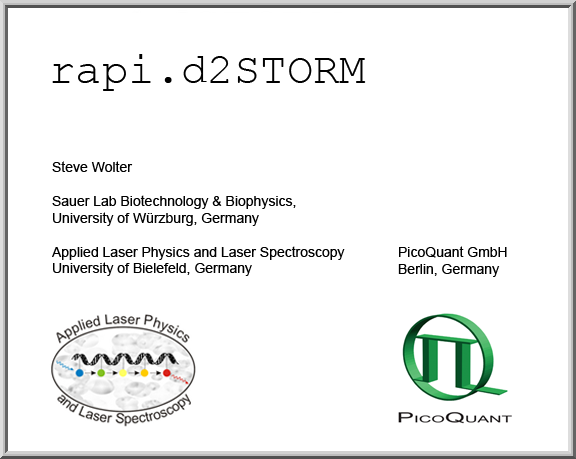
\includegraphics[width=0.205\textwidth]{logo.png} \hspace{10 cm} \includegraphics[width=0.205\textwidth]{klee.jpg}}%\\ Fakult�t f�r Physik}
  \subject {}
  \title {\Large meine LaTeX-Referenz}
  %\author {\sffamily \large vorgelegt von Sven Martin Proppert \vspace {30pt}\\{\small Von der Fakult�t f�r Physik genehmigte}\\Diplom-Arbeit\\{\small zur Erlangung des Grades eines Diplomphysikers.} \vspace {40pt}}
  \author {\sffamily \large vorgelegt von Sven Martin Proppert \vspace {30pt}\\{\small Von der Fakult�t f�r Physik und Astronomie genehmigte}\\Dissertation\\ \vspace {100pt}}
  \date{\today}
  \publishers {\large Gutachter:\\Prof. Dr. rer. nat. Markus Sauer\\Prof. Dr. rer. nat. }
%%end Infos f�r Titlepage
%%end of header



%%your document starts here
\begin{document}
\sffamily				%%schrift serifenlos

\section{Calibration data}

\subsection{record calibration file}
Things needed for recording calibration data\label{tab:reccal}:
\begin{itemize}
	\item thinly coated Tetraspeck surface
	\item objective piezo (e.g. PIfoc, Physik Instrumente)
	\item appropriate cylindrical lens in detection path
\end{itemize}

Exaple procedure:
\begin{enumerate}
	\item place Tetraspeck surface on microscope
	\item set piezo to remote control
	\item focus on Tetraspeck
	\item make the piezo move around focal plane with a triangular function
	\item record data 
	\item exemplary settings piezo:\\
				low position: 45 $\mu$m\\
				high position: 55 $\mu$m\\
				frequence: 0.02 Hz\\
				function: triangular
	\item exemplary camera settings:\\
				exposure time: 0.02 s
\end{enumerate}

\subsection{get calibration curve}
\begin{enumerate}
	\item start rapidstorm, load calibration data to the input field (don't forget to check "`Ignore libtiff warnings"' if your data is a tif-file) and switch to expert mode
	\item "`Size of input pixel"': \\
	enter correct pixelsizes for x and y (to get two fields, click the unjoin button)
	\item "`PSF FWHM"': \textbf{remember your input!} \\
	e.g. Alexa 647: 370 nm
	\item "`Amplitude discarding threshold"': \\
	filters rubbish from data. As your Tetraspeck should be very bright, you would want to enter a high value. 2000-5000 will do for a start
	\item "`Fit window radius"': \textbf{remember your input!} \\
	in order to be able to fit widespread PSFs, enter a value considerably higher than  the PSF FHWM. In our example, the value should be around 1100 nm
	\item "`maximum number of iteration steps for spot fitting"':\\
	\item check boxes "`PSF width is free fit parameter"' and "`Store PSF covariance matrix"'
	\item under "`Output options"' go to the "`Expression filter"' menue\\
		\begin{itemize}
			\item "`value to assign to"':\\
			posz
			\item "`Expression to assign from"':\\
			\textit{X} nm/fr * frame\\
			(in this example: 8 nm/fr *frame)
			\item "`Choose new output"':\\
			"`3D PSF width calibration table"'
		\end{itemize}
	\item go to the "`3D PSF width calibration table"' menue\\
		\begin{itemize}
			\item "`FWHM correction for object size"':\\
			Here, you adjust, how much the PSF FWHM of the Tetraspeck differs from the PSF 				FWHM of a fluorophore in your sample. Our value  - still Voodoo - is 25 nm
			\item "`Number of B spline breakpoints"':\\
			10 should be sufficient in most cases. This setting roughly controls the number 			of basic functions used for fitting.
			\end{itemize}
	\item run evaluation
\end{enumerate}

\par rapidSTORM now created some outputs. You should already know the \textit{filename}.txt and the \textit{filename}-raw.txt (and \textit{filename}.png if you saved the picture. The interesting and new output is \textbf{\textit{filename}-sigma-table.txt}. Plot this file with gnuplot or Origin. As you now tried to get a curve for the whole calibration movie, it is likely that your result will look pretty awful, but that is ok. This is just because the fit routine tried to fit to PSFs which were already too blurred or even showed a first diffraction order. Thus you have to 

\section{Make 3D image of measurement}


%%end is near ;-)
\end{document}


